\documentclass[11pt]{article}

% common LaTeX macros
%
% Last modified: 03-02-2007
%

\usepackage{times}
%-------------------------
% the following magic makes the tt font in math mode be the same as the
% normal tt font (i.e., Courier)
%
\SetMathAlphabet{\mathtt}{normal}{OT1}{pcr}{n}{n}
\SetMathAlphabet{\mathtt}{bold}{OT1}{pcr}{bx}{n}
%-------------------------

\usepackage{amsmath}
\usepackage{amssymb} % for \pitchfork

\newcommand{\NOTE}[1]{%
  \par\leavevmode\noindent\textbf{[[ #1 ]]}\par\leavevmode\noindent}
\newcommand{\CUT}[1]{}
\newcommand{\SIDENOTE}[1]{%
  \marginpar{\tiny\raggedright{#1}}}

\newcommand{\appref}[1]{Appendix~\ref{#1}}
\newcommand{\chapref}[1]{Chapter~\ref{#1}}
\newcommand{\secref}[1]{Section~\ref{#1}}
\newcommand{\tblref}[1]{Table~\ref{#1}}
\newcommand{\figref}[1]{Figure~\ref{#1}}
\newcommand{\listingref}[1]{Listing~\ref{#1}}
\newcommand{\pref}[1]{{page~\pageref{#1}}}
\newcommand{\defref}[1]{Definition~\ref{#1}}
\newcommand{\ruleref}[1]{Rule~\ref{#1}}

\newcommand{\eg}{{\em e.g.}}
\newcommand{\cf}{{\em cf.}}
\newcommand{\ie}{{\em i.e.}}
\newcommand{\etc}{{\em etc.\/}}
\newcommand{\naive}{na\"{\i}ve}
\newcommand{\ala}{{\em \`{a} la\/}}
\newcommand{\etal}{{\em et al.\/}}
\newcommand{\role}{r\^{o}le}
\newcommand{\vs}{{\em vs.}}
\newcommand{\forte}{{fort\'{e}\/}}

%
% language names
\newcommand{\Cplusplus}{\mbox{C\hspace{-.05em}\raisebox{.4ex}{\tiny\bf ++}}}
\newcommand{\Cmm}{\mbox{C\hspace{-.05em}\raisebox{.4ex}{\small\textbf{{-}{-}}}}}
\newcommand{\csharp}{\textsc{C\#}}
\newcommand{\C}{\textsc{C}}
\newcommand{\Ckit}{\textsc{Ckit}}
\newcommand{\java}{\textsc{Java}}
\newcommand{\loom}{\textsc{Loom}}
\newcommand{\moby}{\textsc{Moby}}
\newcommand{\minimoby}{\textsc{MiniMoby}}
\newcommand{\micromoby}{\textsc{microMoby}}
\newcommand{\MOC}{\textsc{MOC}}
\newcommand{\ml}{\textsc{ML}}
\newcommand{\sml}{\textsc{SML}}
\newcommand{\smlnj}{\textsc{SML/NJ}}
\newcommand{\mlj}{\textsc{MLj}}
\newcommand{\cml}{\textsc{CML}}
\newcommand{\pml}{\textsc{PML}}
\newcommand{\ocaml}{\textsc{OCaml}}
\newcommand{\mlkk}{\textsc{ML2000}}
\newcommand{\haskell}{\textsc{Haskell}}
\newcommand{\mltwok}{\textsc{ML2000}}
\newcommand{\scala}{\textsc{Scala}}
\newcommand{\perl}{\textsc{Perl}}
\newcommand{\scheme}{\textsc{Scheme}}
\newcommand{\unix}{\textsc{Unix}}
\newcommand{\smalltalk}{\textsc{Smalltalk}}
\newcommand{\self}{\textsc{Self}}

%
% font commands
\providecommand{\bftt}[1]{{\ttfamily\bfseries{}#1}}
\providecommand{\ittt}[1]{{\ttfamily\itshape{}#1}}
\providecommand{\kw}[1]{\bftt{#1}}
\providecommand{\nt}[1]{{\rmfamily\itshape{#1}}}
\providecommand{\term}[1]{{\sffamily{#1}}}
%
% math-mode versions
\providecommand{\mkw}[1]{\ensuremath{\text{\kw{#1}}}}
\providecommand{\mnt}[1]{\ensuremath{\text{\nt{#1}}}}
\providecommand{\mterm}[1]{\ensuremath{\text{\term{#1}}}}

% braces (in math mode)
\newcommand{\LCB}{\mkw{\{}}
\newcommand{\RCB}{\mkw{\}}}

% underscore
\newcommand{\US}{\char`\_}

%%%%%
% Some common math notation
%

% double brackets
\newcommand{\LDB}{\ensuremath{[\mskip -3mu [}}
\newcommand{\RDB}{\ensuremath{]\mskip -3mu ]}}

\newcommand{\dom}{\ensuremath{\mathrm{dom}}}
\newcommand{\rng}{\ensuremath{\mathrm{rng}}}

% sets
\newcommand{\SET}[1]{\ensuremath{\{#1\}}}
\newcommand{\Fin}{\textrm{Fin}}     % finite power set
\newcommand{\DISJOINT}[2]{\ensuremath{#1 \pitchfork #2}}
\newcommand{\finsubset}{\mathrel{\stackrel{\textrm{fin}}{\subset}}}


% finite maps
\newcommand{\finmap}{\mathrel{\stackrel{\textrm{fin}}{\rightarrow}}}
\newcommand{\MAP}[2]{\SET{#1 \mapsto #2}}
\newcommand{\EXTEND}[2]{\ensuremath{#1{\pm}#2}}
\newcommand{\EXTENDone}[3]{\EXTEND{#1}{\MAP{#2}{#3}}}
\newcommand{\SUBST}[3]{\ensuremath{#1[#2\mapsto{}#3]}}
\newcommand{\SUBSTTWO}[5]{\ensuremath{#1[#2\mapsto{}#3,#4\mapsto{}#5]}}


% timestamp
\newcount\timeHH
\newcount\timeMM
\timeHH=\time
\divide\timeHH by 60
\timeMM=\time
\count255=\timeHH
\multiply\count255 by -60 \advance\timeMM by \count255
\newcommand{\timestamp}{%
  \today{} ---
  \ifnum\timeHH<10 0\fi\number\timeHH\,:\,\ifnum\timeMM<10 0\fi\number\timeMM}


\usepackage{graphicx}
\usepackage{../common/code}

\title{Manticore Implementation Note \\ Runtime initialization}
\author{The Manticore Group}
\date{Draft of \today}

\begin{document}
\maketitle

\section{Overview}
This note describes the initialization protocol of our runtime system. \figref{fig:runtime-initialization} 
gives an overview of our initialization process. The first three steps occur in the C runtime. For each VProc
we allocate memory, initialize state, and finally spawn a PThread. The first VProc then 
executes some Manticore code to bootstrap the schedulers. Other VProcs start in an idle state. When the
boostrapping finishes, the first VProc wakes the other VProcs and the main computation begins. 

\begin{figure}[t]
  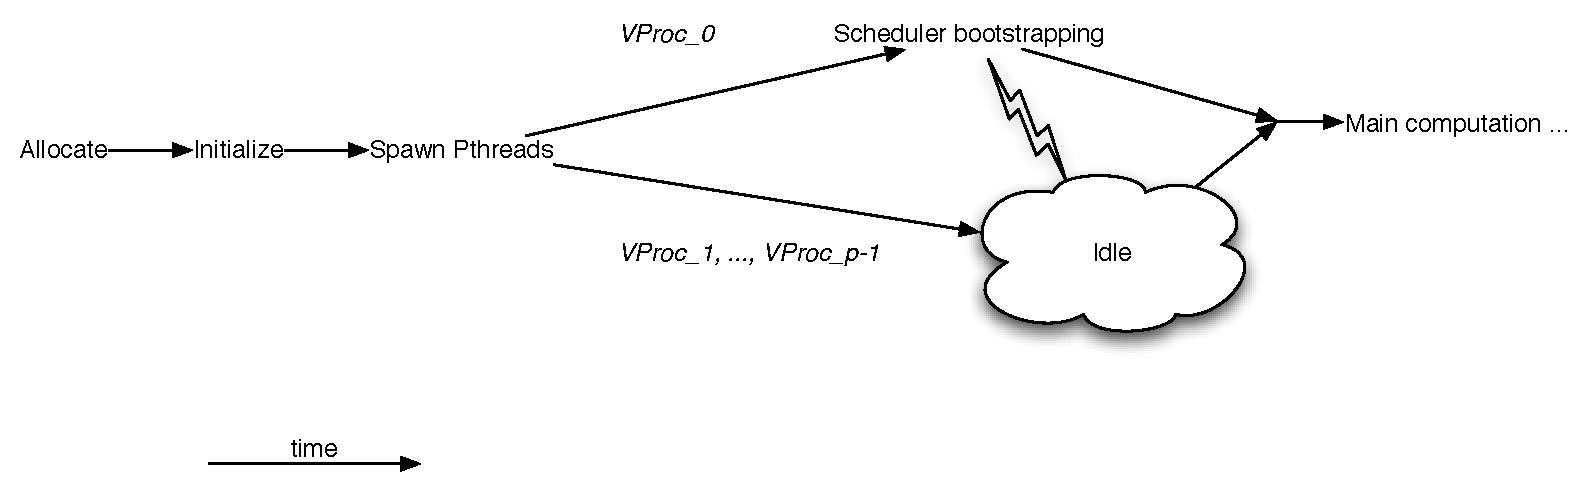
\includegraphics[scale=0.45]{pictures/runtime-initialization.pdf}
  \label{fig:runtime-initialization}
\end{figure}

The rest of this note describes some subtle aspects of the initialization protocol.

\section{Three types of Pthreads}
During initialization, our C runtime creates three types of Pthreads.
\begin{enumerate}
  \item The \textbf{``ping'' thread} simulates timer interrupts by sendings periodic signals to VProcs.
  \item The \textbf{lead VProc} begins executing PML code.
  \item The \textbf{subordinate VProcs} immediately go idle (there are $p-1$ of these Pthreads).
\end{enumerate}

\section{The trampoline}
\label{sec:trampoline}
The trampoline is a per-VProc mechanism that lets the C runtime pass signals to the scheduler stack. The 
trampoline is a continuation that consumes either a nil value or a fiber. 
\begin{centercode}
val trampoline : fiber option cont
\end{centercode}
A nil value indicates that the VProc has awoken from an idle state; a fiber indicates that a 
preemption has occured.
Our bootstrapping code must initialize the trampoline before any scheduling code can run. The
\texttt{SchedulerUtils} module contains our initialization code.

\section{The scheduler-action stack}
\label{sec:action-stack}
During bootstrapping, we seed each VProc with a separate instance of the top-level scheduler. This code
is part of the \texttt{SchedulerUtils} module.

\section{Bootstrapping the top-level scheduler}
The final step of initialization is bootstrapping the top-level scheduler. This process sets the trampoline
(\secref{sec:trampoline}), initializes the scheduler-action stacks (\secref{sec:action-stack}), and then
wakes up the idle VProcs.
At this point, the user's computation can start executing.

This code is part of the \texttt{SchedulerUtils} module.

\section{Idle VProcs}
\begin{itemize}
  \item Each subordinate VProc begins in an idle state.
  \item VProcs go idle by invoking the \texttt{VProc.@wait} operation.
  \item There are two ways to wake an idle VProc:
    \begin{enumerate}
      \item Send the VProc a messenger thread.
      \item Enqueue a thread on the VProc.
    \end{enumerate}
  \item After waking up, we must unload the landing pad. If we fail to do so, scheduling code will almost
    certainly find that the VProc queue is empty, and therefore will switch back to an idle state. This
    situation can cause the computation to diverge.
\end{itemize}

\end{document}

